%% Thesis summary in IEEE conference style.
%% Compile from within the "riassunto/" folder:
%%   pdflatex riassunto.tex
%%   pdflatex riassunto.tex
%% (IEEEtran.cls is shipped locally in this folder; images are referenced
%%  relative to the main thesis project via ../immagini and ../evaluation.)

\documentclass[conference]{IEEEtran}

\usepackage[T1]{fontenc}
\usepackage[utf8]{inputenc}
\usepackage{graphicx}
\usepackage{amsmath,amssymb}
\usepackage{booktabs}
\usepackage{eurosym}
\usepackage{url}
\usepackage[hidelinks]{hyperref}

\graphicspath{{../immagini/}{../evaluation/figures/}}

\begin{document}

\title{Migrating Legacy Services to a Cloud-Native\\
Architecture: A Case Study on Outsight Cloud}

\author{\IEEEauthorblockN{Giovanni Russo}
\IEEEauthorblockA{Politecnico di Torino\\
Turin, Italy\\
s343424}}

\maketitle

\begin{abstract}
Legacy platforms often evolve through years of incremental development,
producing architectures that are hard to scale, maintain, and modernize.
This thesis addresses a concrete engineering problem: migrating Outsight
Cloud, a production platform for LiDAR-related workflows, from a legacy
service-oriented setup to a cloud-native architecture on Amazon Web
Services (AWS). The original system ran on DigitalOcean virtual machines
orchestrated with Docker Compose and relied on Airtable as its primary
operational database, an arrangement that progressively caused scalability,
consistency, and operational-governance problems. Rather than a big-bang
rewrite, the thesis proposes and evaluates an incremental migration
strategy based on Infrastructure as Code (Terraform), AWS managed services
(ECS Fargate, RDS PostgreSQL, S3, CloudFront), and progressive coexistence
between legacy and target components. The design is driven by an explicit
decision framework that weighs technical and economic trade-offs. A
reproducible, script-driven benchmark shows that the migration cuts direct
infrastructure cost by 50\% ($-$\euro235/month), reduces mean HTTP
latency by about 38\%, and lowers recurring operational effort by roughly
one order of magnitude, for a combined estimated saving near
\euro17{,}000/year.
\end{abstract}

\begin{IEEEkeywords}
cloud migration, cloud-native, AWS, Infrastructure as Code, Terraform,
ECS Fargate, PostgreSQL, legacy modernization
\end{IEEEkeywords}

\section{Introduction}
Cloud computing has changed how software systems are designed, deployed,
and operated. Managed services, elastic infrastructure, and deployment
automation are hard to reproduce in self-managed environments, and many
organizations are therefore modernizing legacy applications toward
cloud-native architectures. Migrating a production platform, however, is
rarely straightforward: legacy systems accumulate architectural
dependencies and operational habits that complicate scalability and
long-term evolution.

This work studies the migration of \emph{Outsight Cloud} (OC), a platform
that manages LiDAR-related workflows, simulations, organizations, and
sites. Before the migration, OC ran on DigitalOcean Droplets orchestrated
through Docker Compose and depended on several external services, most
notably Airtable as its operational datastore. This stack enabled fast
early development but, as usage and integrations grew, it showed clear
architectural strain.

The central engineering objective is to migrate OC to a managed cloud
environment while regaining explicit ownership of core data and
infrastructure assets. The main design choice of the whole project is
\emph{incrementality}: every architectural change is made independently
verifiable, so modernization proceeds through controlled steps rather than
a single high-risk cutover. This principle is the recurring theme of the
thesis, and it is what makes the migration safe to run against a live
production system.

\section{Problem and Background}
Outsight Cloud combined self-managed virtual machines with a set of
external service dependencies. Airtable, in particular, had grown from a
simple datastore into a critical dependency embedded in application logic
and operational workflows. From this baseline, four concrete problems
follow.

\textbf{Weak data model.} Relationships between organizations, sites,
simulations, and permissions were expressed through linked records and
lookup fields rather than relational constraints. Consistency depended on
application-side logic, and the same logical field could appear as a scalar
or an array depending on context, increasing backend complexity.

\textbf{Operational fragility.} Deployments were performed by SSH-ing into
Droplets and restarting Docker Compose, with no atomic rollback, no
auto-scaling, and no centralized observability. Routine maintenance
(OS patching, capacity planning, incident diagnosis) fell entirely on the
engineering team.

\textbf{Cost and coupling.} Airtable's per-seat pricing (\euro294/month for
seven editor licences) was ill-suited to an infrastructure role, while
vendor-specific concepts reduced architectural flexibility.

\textbf{Migration risk.} The platform served production traffic, so it
could not tolerate a long interruption or an irreversible switch.

Related work frames the solution space. Newman argues against big-bang
rewrites and in favour of incremental delivery, the strangler-fig pattern,
and parallel runs~\cite{newman2021building}. Morris describes Infrastructure
as Code and the expand-and-contract pattern for changing live systems
safely~\cite{morris2021iac}. Cloud migration is commonly classified as
rehosting, replatforming, or refactoring~\cite{awsCloudMigrationOverview}.
The OC migration is best described as a hybrid: replatforming the runtime
(Docker Compose~$\rightarrow$~ECS Fargate) combined with selective
refactoring of the data layer (Airtable~$\rightarrow$~PostgreSQL) and the
introduction of IaC. Existing guidance, however, tends to treat technical
architecture and economic sustainability separately, and provides limited
evidence on intermediate validation. This thesis fills that gap with a
decision-oriented case study backed by quantitative evaluation.

\section{Solution Design}
The migration design was driven by an explicit decision framework rather
than by technology preference. Cloud providers (AWS, Azure, GCP,
DigitalOcean, on-premises) and container runtimes (Kubernetes vs.\ ECS
Fargate) were compared against technical and economic criteria: managed
services fit, IaC and automation support, operational complexity, ecosystem
maturity, and continuity with the existing baseline.

\textbf{Runtime.} Kubernetes was evaluated but rejected for this stage:
its cluster-management overhead (networking, upgrades, monitoring, capacity
planning, security governance) was not justified by the scale of
OC~\cite{kubernetesOverview}, echoing Newman's caution against premature
platform complexity~\cite{newman2021building}. \textbf{Amazon ECS Fargate}
was selected because it runs standard Docker containers with no worker
nodes to manage, easing the transition from Docker Compose.

\textbf{Provider.} AWS was chosen for the maturity of its managed-service
ecosystem, its strong Terraform integration, and its alignment with the
company's broader cloudification direction. The acknowledged trade-off is
that AWS can become expensive under specific scaling conditions, but the
balance of service quality, flexibility, and migration continuity favoured
it.

The resulting target architecture (Fig.~\ref{fig:aws}) follows a layered
model: a delivery layer (browser, CloudFront), a routing layer (Application
Load Balancer), an application layer (Vue frontend and Node.js backend on
ECS Fargate), and a managed-services layer (RDS PostgreSQL, Redis, S3,
Cognito, SES, SNS). PostgreSQL replaces Airtable as the primary datastore,
restoring an explicit relational schema with database-level integrity.
Static assets live in a private S3 bucket exposed only through CloudFront
Origin Access Control, while ACM manages TLS centrally. Security groups
ensure that containers accept traffic only from the ALB.

\begin{figure}[!t]
\centering
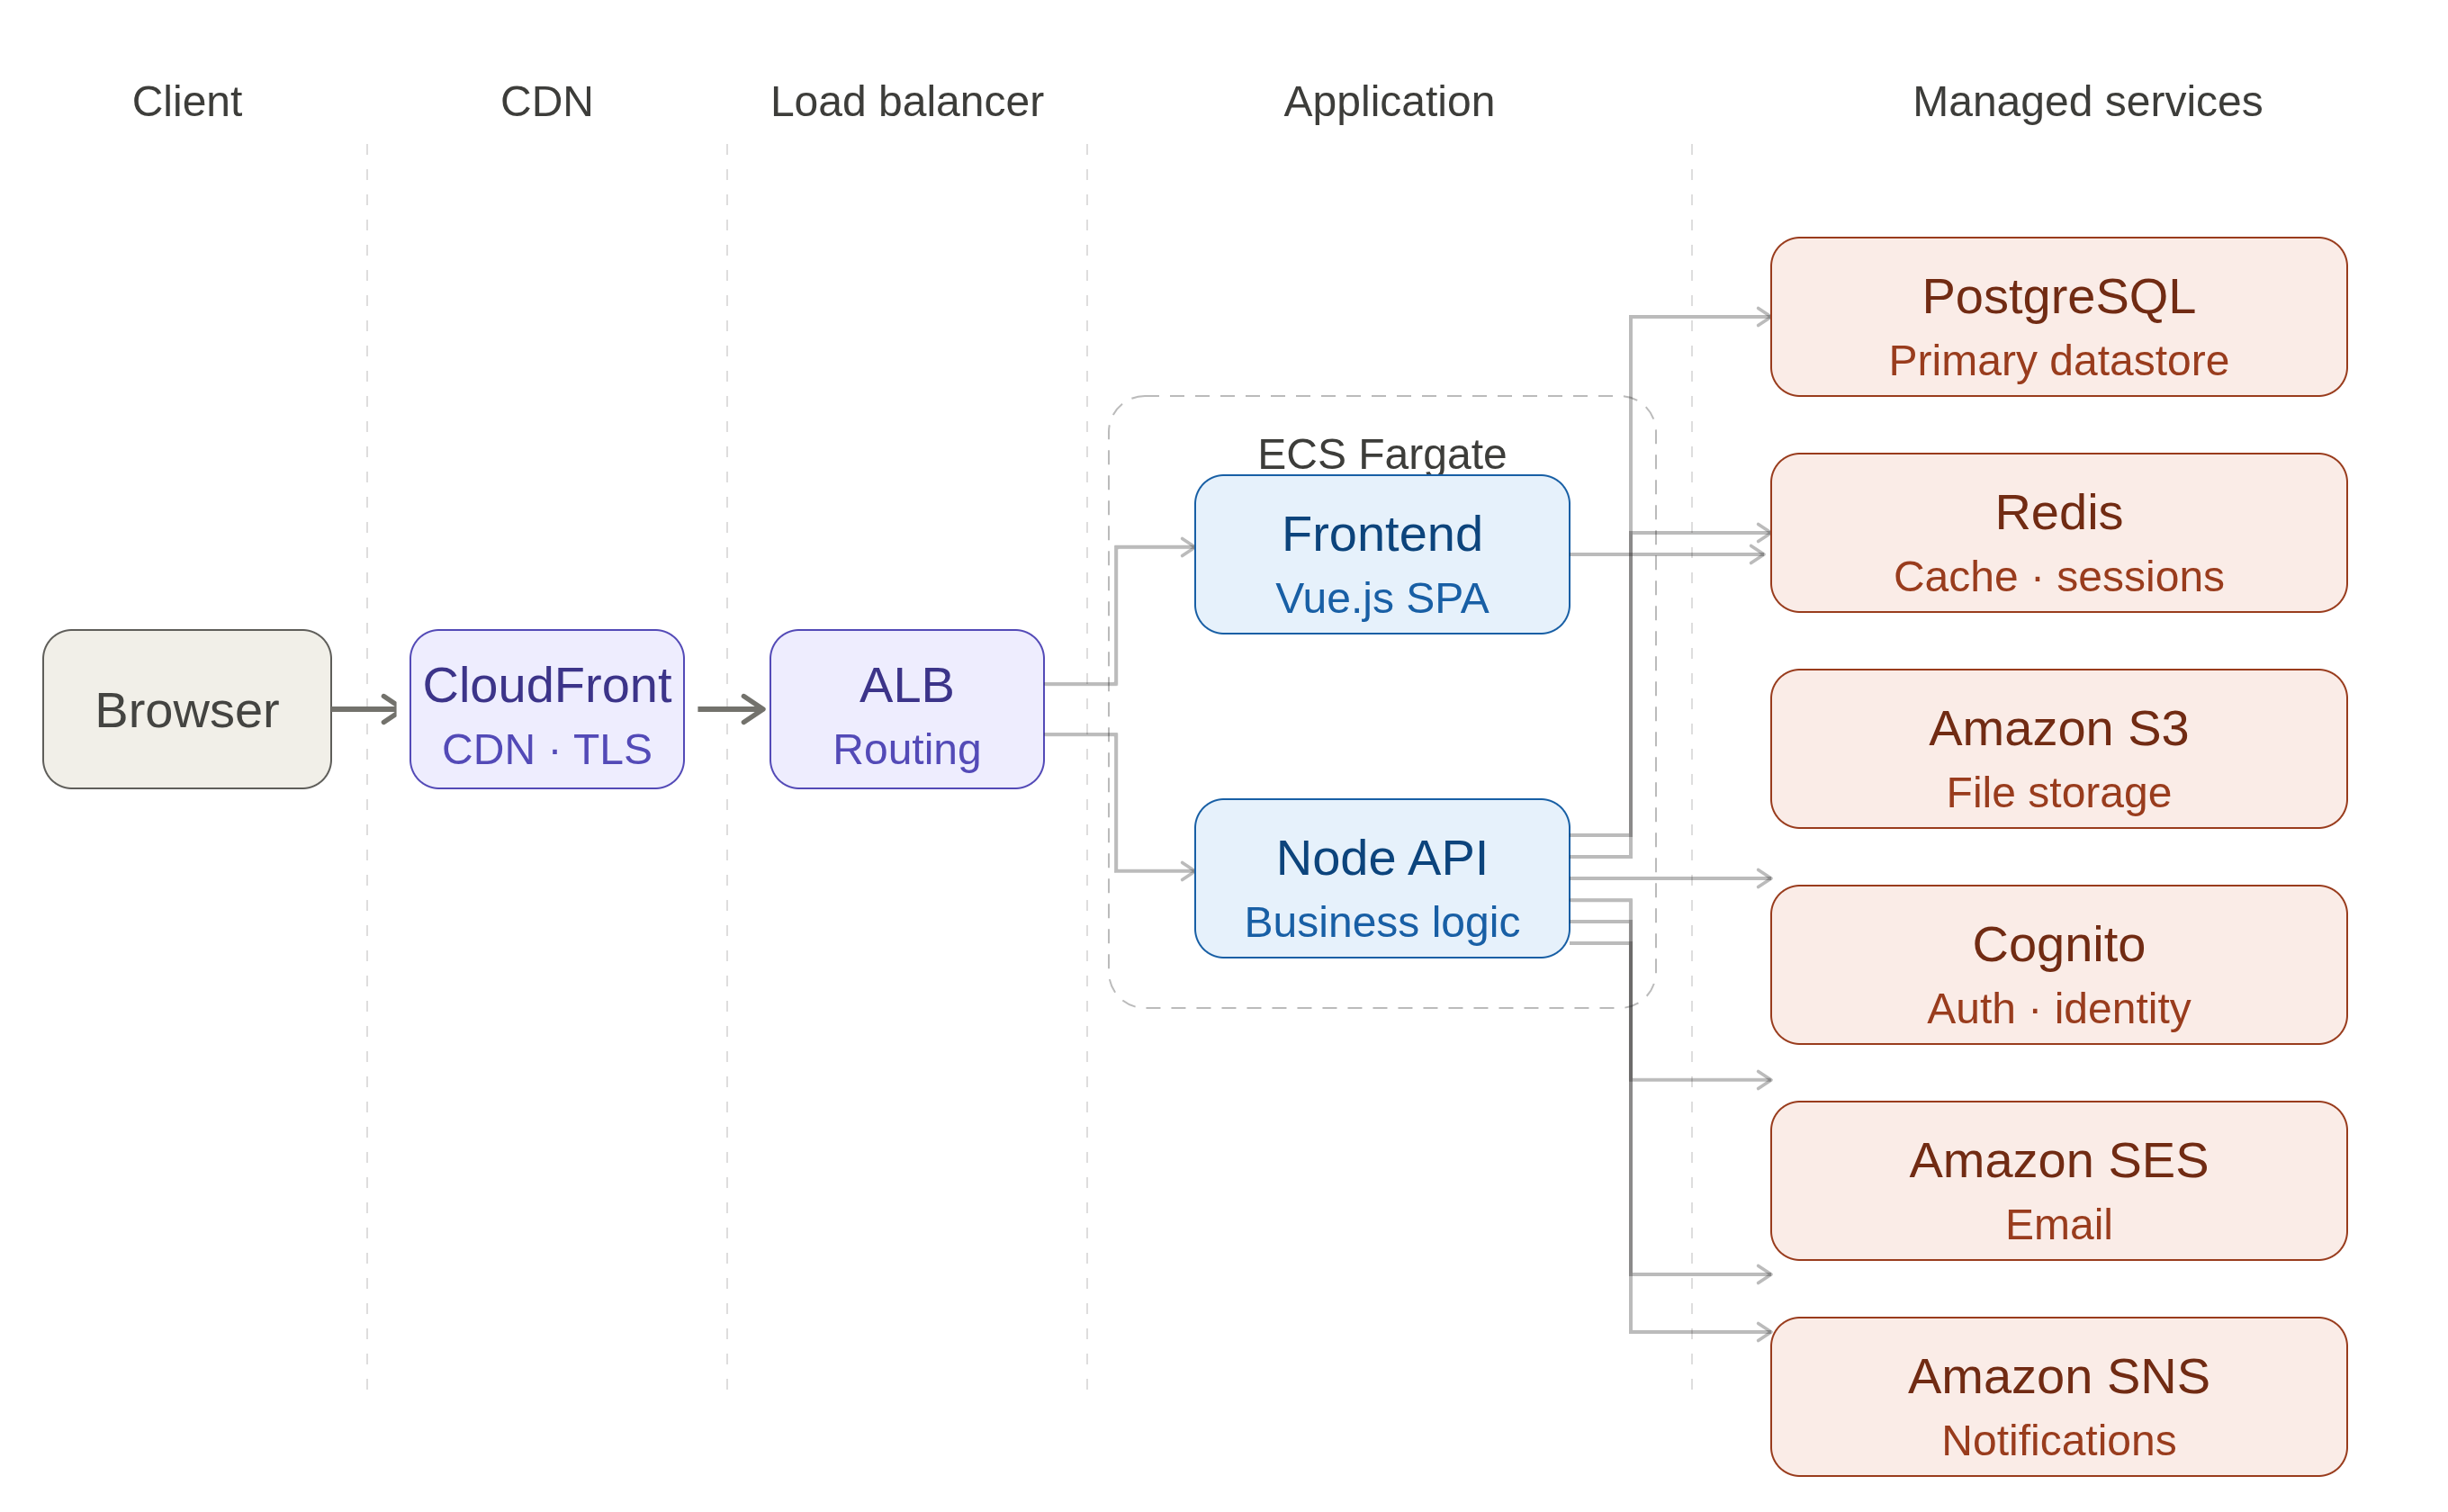
\includegraphics[width=\columnwidth]{outsight_aws_architecture.png}
\caption{Target AWS architecture. Requests flow from the browser through
CloudFront and the Application Load Balancer to the Vue and Node.js
services on ECS Fargate, which integrate with managed services
(RDS PostgreSQL, Redis, S3, Cognito, SES, SNS).}
\label{fig:aws}
\end{figure}

\section{Implementation}
The migration was executed as four independently verifiable tracks:
(i)~establish the AWS environment, (ii)~formalize provisioning with
Terraform, (iii)~migrate data from Airtable to PostgreSQL, and
(iv)~validate data, application behaviour, and deployment before
production switchover. Sequencing the work this way kept the migration
traceable and limited the blast radius of any single change.

\textbf{Infrastructure as Code.} The whole target stack (ECS services,
ALB, Route~53 records, ACM certificates, CloudWatch log groups, and
S3/CloudFront) was defined declaratively in Terraform, following Morris's
core practices: define everything as code, test continuously, and build
small loosely coupled pieces~\cite{morris2021iac,hashicorpTerraformIntro}.
The write--plan--apply workflow allowed each change to be reviewed before
execution, and shared state enabled drift detection. Registry credentials
were injected at runtime through AWS Secrets Manager instead of being
embedded in Terraform state.

\textbf{Coexistence and validation.} Routing responsibilities moved from
Traefik to the ALB, and the backend was adapted so its external routes
matched the ALB model. Dedicated scripts replicated data from Airtable into
PostgreSQL and validated consistency through machine-readable reports,
turning data migration into a repeatable, verifiable workflow. Development
and production concerns were kept separate, and the final switchover was
performed gradually through Route~53 DNS updates, avoiding a single
disruptive cutover across infrastructure, routing, and storage.

\section{Evaluation}
The migration was evaluated with a reproducible, script-driven benchmark
along three dimensions: direct infrastructure cost, end-to-end HTTP
latency, and recurring operational effort. Latency was measured with
\texttt{curl} timing variables over $N=100$ independent requests per
environment, issued from the same client in Paris with fresh connections
(no keep-alive), and summarized with 95\% confidence intervals.

\textbf{Cost.} The legacy platform cost \euro466/month (DigitalOcean
Droplets \euro102, Spaces \euro70, Airtable \euro294). The AWS platform
costs \euro231/month, a \textbf{50\% reduction} (Fig.~\ref{fig:cost}).
The saving is structural: Airtable (\euro294) is replaced by Amazon RDS
(\euro48), an 84\% cut in the database category, while object storage drops
89\% (S3 \euro8 vs.\ Spaces \euro70).

\begin{figure}[!t]
\centering
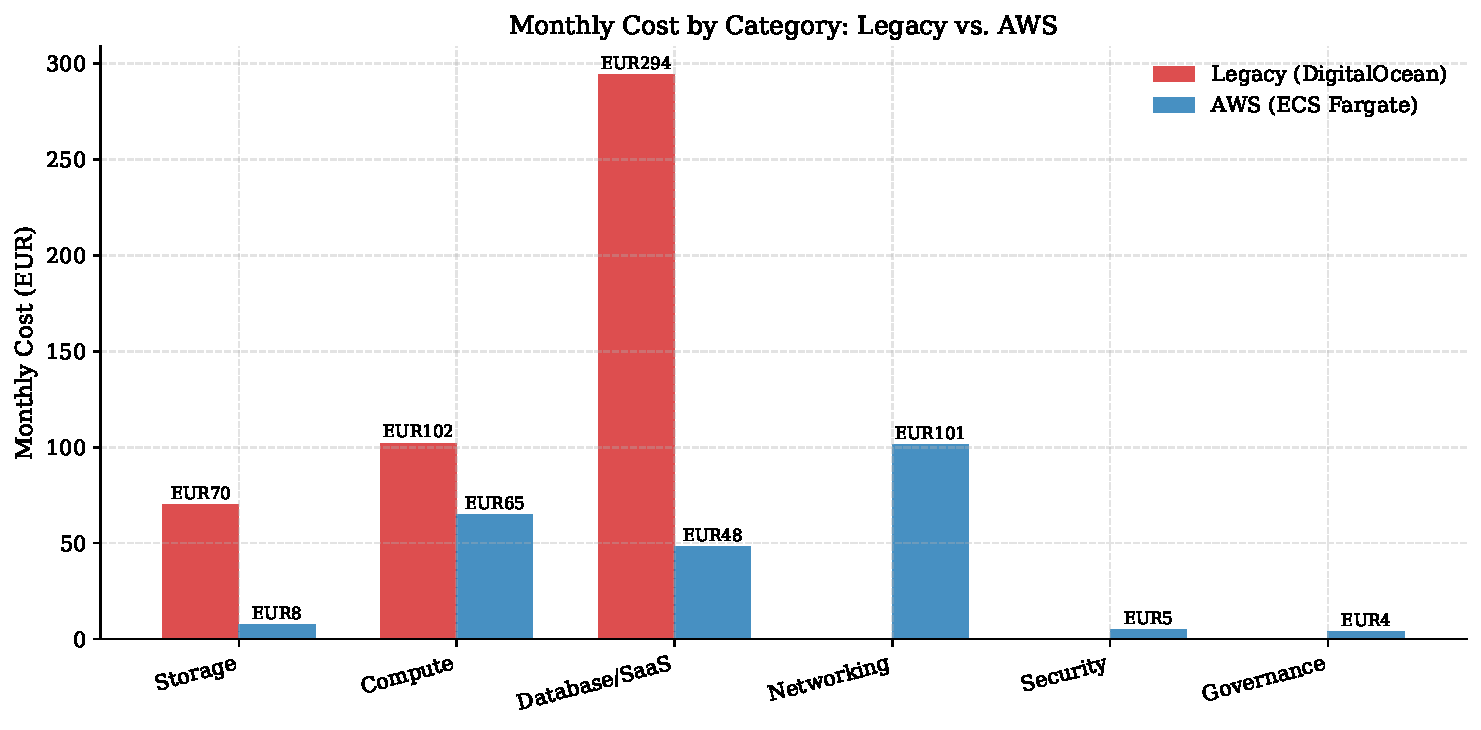
\includegraphics[width=\columnwidth]{cost_bar_comparison.pdf}
\caption{Monthly cost by category, legacy vs.\ AWS. Categories absent from
the legacy platform (load balancer, networking, security) appear as zero.}
\label{fig:cost}
\end{figure}

\textbf{Latency.} The AWS architecture reduces every HTTP timing component
(Fig.~\ref{fig:latency}). DNS and TCP fall by about 89\%, thanks to
Route~53 anycast and CloudFront points of presence; the TLS handshake drops
48\% (85\,ms~$\rightarrow$~44\,ms) via TLS~1.3 and session resumption. The
user-perceived Time to First Byte (TTFB) falls 38\% (131\,ms~$\rightarrow$~81\,ms),
and the AWS 95th-percentile TTFB (105\,ms) is lower than the legacy
\emph{median} (125\,ms). Beyond the mean, the distribution becomes much
tighter: the long tail of the legacy platform (TTFB up to ~395\,ms)
disappears, so the worst-case user experience is now close to the median.

\begin{figure}[!t]
\centering
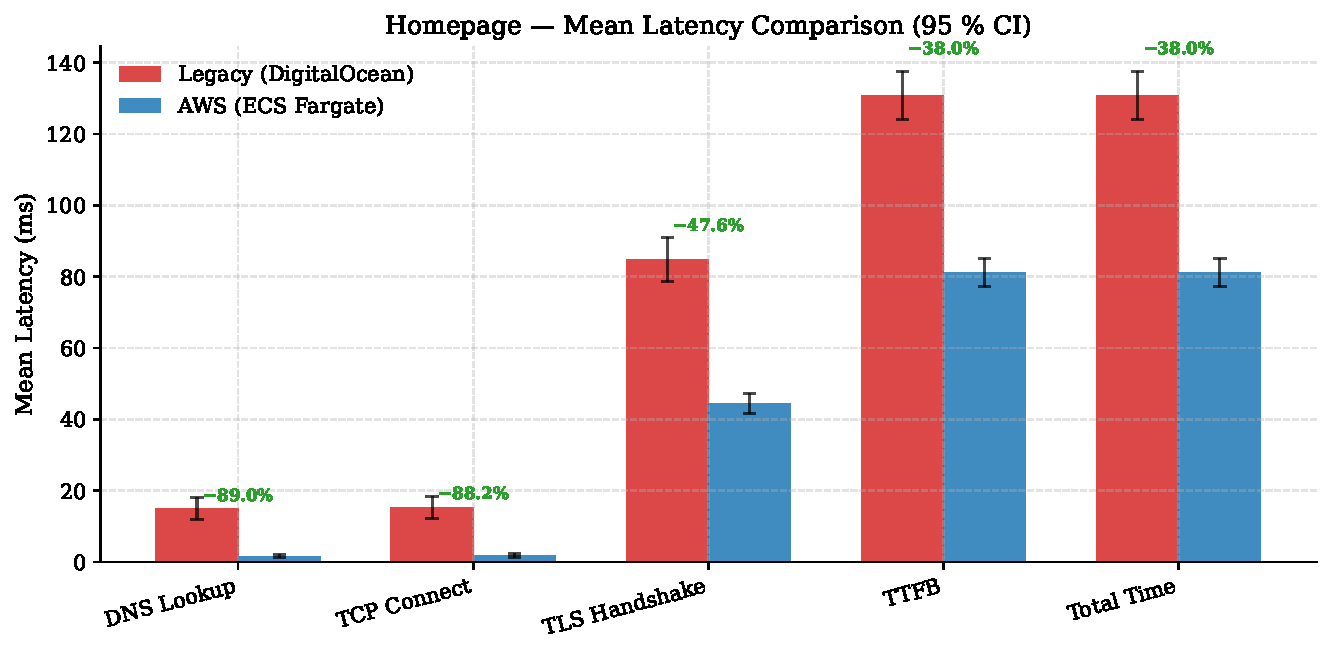
\includegraphics[width=\columnwidth]{home_bar_comparison.pdf}
\caption{Mean latency per HTTP timing component, legacy vs.\ AWS, with 95\%
CI error bars and percentage improvement.}
\label{fig:latency}
\end{figure}

\textbf{Operational effort.} Delegating patching, scaling, deployment, and
database administration to managed services reduces recurring operational
work from an estimated 13--20\,h/month to 1.5--2\,h/month. At a conservative
\euro80/h loaded rate, this is a further \euro1{,}180/month saving on
engineering time. Combined with the \euro235/month infrastructure saving,
the migration yields roughly \euro1{,}415/month, about \euro17{,}000/year.
This roughly 90\% drop in operational effort is consistent with independent
industry evidence: a Forrester Total Economic Impact study commissioned by
AWS reports around 97.5\% provisioning time savings, a 30\% DevOps
productivity gain, and a 90\% reduction in high-priority incidents after
adopting managed cloud operations~\cite{forresterTeiCloudOps}.
Table~\ref{tab:results} collects the main results.

\begin{table}[!t]
\caption{Main evaluation results}
\label{tab:results}
\centering
\begin{tabular}{ll}
\toprule
\textbf{Metric} & \textbf{Result} \\
\midrule
Infrastructure cost & \euro466 $\rightarrow$ \euro231/mo ($-$50\%) \\
Database (Airtable$\rightarrow$RDS) & \euro294 $\rightarrow$ \euro48/mo ($-$84\%) \\
Object storage (Spaces$\rightarrow$S3) & \euro70 $\rightarrow$ \euro8/mo ($-$89\%) \\
Mean TTFB & 131 $\rightarrow$ 81\,ms ($-$38\%) \\
DNS / TCP latency & $\approx-$89\% \\
Operational effort & 13--20 $\rightarrow$ 1.5--2\,h/mo \\
Combined saving & $\approx$\euro1{,}415/mo ($\approx$\euro17k/yr) \\
\bottomrule
\end{tabular}
\end{table}

\section{Conclusion}
This thesis showed that a legacy-to-cloud-native migration is most
effective when treated as a structured engineering process rather than a
simple relocation. An explicit decision framework selected AWS managed
services and ECS Fargate over more complex or less aligned alternatives; an
IaC-first, incremental strategy with dual-backend coexistence and automated
validation made each step independently verifiable and reversible. The
quantitative evaluation confirms measurable gains across all three
dimensions: 50\% lower infrastructure cost, ~38\% lower mean latency with a
much tighter distribution, and roughly a tenfold reduction in operational
effort.

The work also has clear limits. The latency benchmark targets the public
homepage endpoint; authenticated API and database-intensive workflows were
not measured. Operational figures are informed estimates rather than
recorded timesheets, and steady-state latency was measured under sequential
rather than concurrent load. These points define natural future work:
extending benchmarks to authenticated and database-heavy paths, load and
scalability testing of Fargate auto-scaling and RDS pooling, deeper IAM
standardization with Cognito, and richer observability. Beyond OC, the
decision framework, IaC-first provisioning, dual-backend validation, and
incremental rollout planning are transferable to other legacy modernization
scenarios.

\begin{thebibliography}{1}
\bibitem{newman2021building}
S.~Newman, \emph{Building Microservices: Designing Fine-Grained Systems},
2nd~ed. O'Reilly Media, 2021.

\bibitem{morris2021iac}
K.~Morris, \emph{Infrastructure as Code: Dynamic Systems for the Cloud Age},
2nd~ed. O'Reilly Media, 2021.

\bibitem{awsCloudMigrationOverview}
Amazon Web Services, ``What is cloud migration?,'' 2026. [Online].
Available: \url{https://aws.amazon.com/what-is/cloud-migration/}

\bibitem{kubernetesOverview}
The Kubernetes Authors, ``Overview of Kubernetes,'' 2026. [Online].
Available: \url{https://kubernetes.io/docs/concepts/overview/}

\bibitem{hashicorpTerraformIntro}
HashiCorp, ``What is Terraform?,'' 2026. [Online]. Available:
\url{https://developer.hashicorp.com/terraform/intro}

\bibitem{forresterTeiCloudOps}
Forrester Consulting, ``The Total Economic Impact of AWS Cloud Operations,''
Total Economic Impact study commissioned by AWS, May 2022.
\end{thebibliography}

\end{document}
